\documentclass[12pt]{article}

\input quiz-setup
\newcommand{\version}{} 
\newcommand{\xzero}{}
\newcommand{\xone}{}
\newcommand{\xtwo}{}
\newcommand{\xthree}{}
\newcommand{\xfour}{}
\newcommand{\xfive}{}

\newcommand{\ExamName}{Quiz \#5\version}
% \newcommand{\CourseName}{Math 34A}
% \renewcommand{\Quarter}{Spring 2017}



\begin{document}
%%
%% Version A:
\renewcommand{\version}{a}
\renewcommand{\xzero}{0.0}
\renewcommand{\xone}{1.3}
\renewcommand{\xtwo}{2.9}
\renewcommand{\xthree}{4.1}
\renewcommand{\xfour}{5.3}
\renewcommand{\xfive}{6.5}
% 
\begin{minipage}{0.25\linewidth}
  \CourseName\ \Quarter \\
  \ExamName \\[1em]
  \textbf{No calculators}\\[2em]
\end{minipage}
\hfill
\begin{minipage}[t]{0.4\linewidth}
  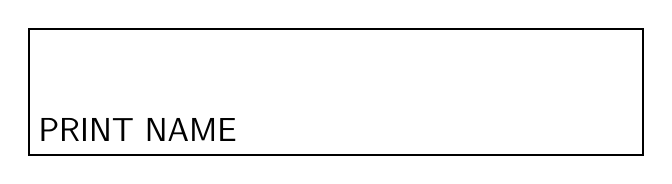
\begin{tikzpicture}[x=26mm,y=16mm]
    \draw[thick,black] (0,0) rectangle (3,1);
    \node[\faintcolor,right] at (0,0.2) {\large\textsf{PRINT NAME}};
  \end{tikzpicture}
\end{minipage}
\hfill
\begin{minipage}{0.25\linewidth}
  \vspace*{-3.25em}
  \ \hfill
  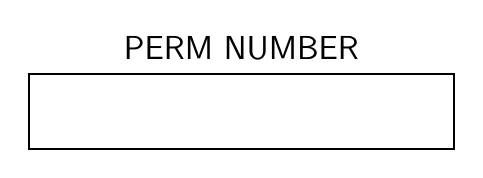
\begin{tikzpicture}[x=36mm,y=16mm]
    \node[\faintcolor] at (0.75,0.8) {\large\textsf{PERM NUMBER}};
    \draw[thick,black] (0,0) rectangle (1.5,0.6);
  \end{tikzpicture}
\end{minipage}
% \medskip
\vspace*{-0.25in}

Put your answer in the 
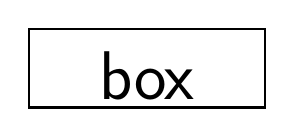
\begin{tikzpicture}[x=10mm,y=10mm,baseline=3mm] 
  \draw[thick,black] (0,0) rectangle (3,1);
  \node[\faintcolor] at (1.5,0.4) {\Huge\textsf{box}};
\end{tikzpicture}
provided.
\hfill
\begin{minipage}{0.5\linewidth}
  \textbf{TA:}\ 
  \parbox[t]{0.7in}{%
    \checkbox\ \TAOne \\
    \checkbox\ \TATwo 
  }
  \parbox[t]{0.7in}{%
    \checkbox\ \TAThree\\
    \ \ \ 
  }
  % \ 
  % \parbox[t]{4in}{%
  % \textbf{Section Time:}
  \hfill%\hspace*{0.25in}
  % \ 
  % \parbox[t]{4in}{%
  % \textbf{Section Time:}
  \textbf{Time:}
  \parbox[t]{0.55in}{%
    \checkbox\ 8am \\
    \checkbox\ 5pm
  }
  \quad
  \parbox[t]{0.55in}{%
    \checkbox\ 6pm \\
    \checkbox\ 7pm 
  }
  % }
\end{minipage}
\noindent\hspace*{-2em}\rule{\textwidth+4em}{1pt}%

\begin{enumerate}
  \setcounter{problemnumber}{0}
  \Problem
  Andy is out for a run.  The rate at which Andy burns calories
  depends on the pace of his run -- a faster pace burns calories
  quicker.  Let $x$ be his pace, in minutes per kilometer, and $f(x)$ be the
  rate at which he burns calories (in calories per hour) at pace $x$.  
  \begin{enumerate}
    \Part What are the units of $f'(x)$?
    \hfill
    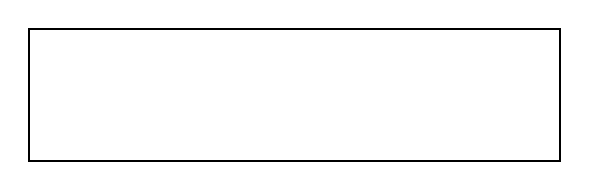
\begin{tikzpicture}[x=25mm,y=12mm,baseline={6mm}]
      \draw[thick,black] (-0.2,-0.2) rectangle (2.5,1.2);
      % \node at (0.1,0.5) {$x=$};
    \end{tikzpicture}
    \vfill

    \Part If $f(x) = 240/x$, what is the average rate of change
    between $x=8$ and $x=10$?
    \hfill
    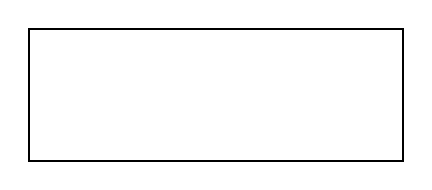
\begin{tikzpicture}[x=25mm,y=12mm,baseline={6mm}]
      \draw[thick,black] (-0.2,-0.2) rectangle (1.7,1.2);
      % \node at (0.1,0.5) {$x=$};
    \end{tikzpicture}
    \vfill
  \end{enumerate}

\end{enumerate}
\newpage
%%
%% Version B:
\renewcommand{\version}{b}
\renewcommand{\xzero}{0.0}
\renewcommand{\xone}{1.4}
\renewcommand{\xtwo}{3.6}
\renewcommand{\xthree}{5.0}
\renewcommand{\xfour}{6.1}
\renewcommand{\xfive}{7.5}
\setcounter{problemnumber}{0}
% 
\begin{minipage}{0.25\linewidth}
  \CourseName\ \Quarter \\
  \ExamName \\[1em]
  \textbf{No calculators}\\[2em]
\end{minipage}
\hfill
\begin{minipage}[t]{0.4\linewidth}
  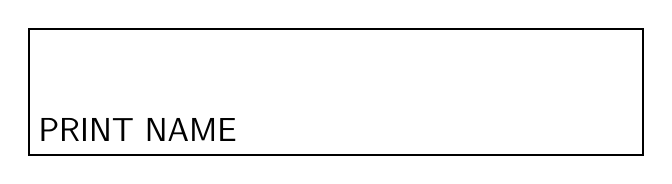
\begin{tikzpicture}[x=26mm,y=16mm]
    \draw[thick,black] (0,0) rectangle (3,1);
    \node[\faintcolor,right] at (0,0.2) {\large\textsf{PRINT NAME}};
    % \node[\faintcolor] at (1.5,0.4) {\Huge\textsf{PRINT NAME}};
  \end{tikzpicture}
\end{minipage}
\hfill
\begin{minipage}{0.25\linewidth}
  \vspace*{-3.25em}
  \ \hfill
  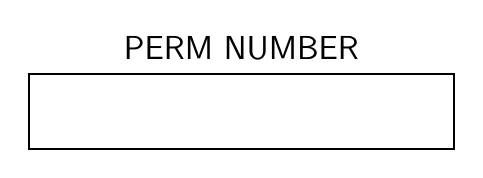
\begin{tikzpicture}[x=36mm,y=16mm]
    \node[\faintcolor] at (0.75,0.8) {\large\textsf{PERM NUMBER}};
    \draw[thick,black] (0,0) rectangle (1.5,0.6);
  \end{tikzpicture}
\end{minipage}
% \medskip
\vspace*{-0.45in}

\begin{minipage}{0.45\linewidth}
  Put your answer in the 
  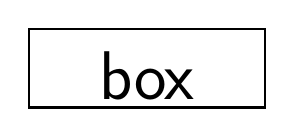
\begin{tikzpicture}[x=10mm,y=10mm,baseline=3mm] 
    \draw[thick,black] (0,0) rectangle (3,1);
    \node[\faintcolor] at (1.5,0.4) {\Huge\textsf{box}};
  \end{tikzpicture}
  provided.
\end{minipage}
\hfill
\begin{minipage}{0.5\linewidth}
  \textbf{TA:}\ 
  \parbox[t]{0.85in}{%
    \checkbox\ \TAThree \\
    \checkbox\ \TAOne %  \\
  }
  \parbox[t]{0.85in}{%
    \checkbox\ \TATwo
  }
  \textbf{Time:}
  \parbox[t]{0.55in}{%
    \checkbox\ 8am \\
    \checkbox\ 5pm
  }
  \quad
  \parbox[t]{0.55in}{%
    \checkbox\ 6pm \\
    \checkbox\ 7pm 
  }
  % }
\end{minipage}
\noindent\hspace*{-2em}\rule{\textwidth+4em}{1pt}%

\begin{enumerate}
  \setcounter{problemnumber}{0}
  \Problem %\Points{3} %
  Andi is out for a run.  The rate at which Andi burns calories
  depends on the pace of her run -- a faster pace burns calories
  quicker.  Let $x$ be her pace, in minutes per mile, and $f(x)$ be the
  rate at which she burns calories (in calories per hour) at pace $x$.  
  \begin{enumerate}
    \Part What are the units of $f'(x)$?
    \hfill
    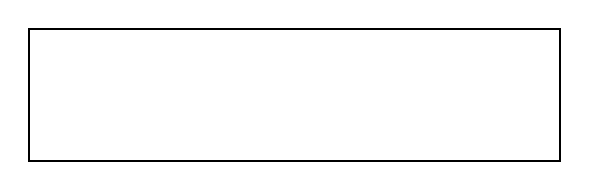
\begin{tikzpicture}[x=25mm,y=12mm,baseline={6mm}]
      \draw[thick,black] (-0.2,-0.2) rectangle (2.5,1.2);
      % \node at (0.1,0.5) {$x=$};
    \end{tikzpicture}
    \vfill

    \Part If $f(x) = 300/x$, what is the average rate of change
    between $x=10$ and $x=15$?
    \hfill
    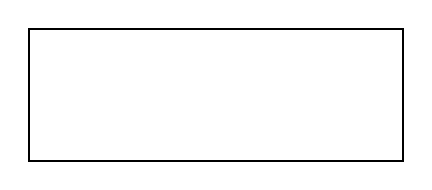
\begin{tikzpicture}[x=25mm,y=12mm,baseline={6mm}]
      \draw[thick,black] (-0.2,-0.2) rectangle (1.7,1.2);
      % \node at (0.1,0.5) {$x=$};
    \end{tikzpicture}
    \vfill


  \end{enumerate}


\end{enumerate}



\end{document}
